% Asset ID: A22FurtherKinematicsTikZ-001
% Unit: A22
% Topic: Further Kinematics
% Related section: Constant velocity vector motion
\documentclass[tikz,border=8pt]{standalone}
\usepackage{amsmath}
\usetikzlibrary{arrows.meta,positioning,angles,quotes}
\begin{document}

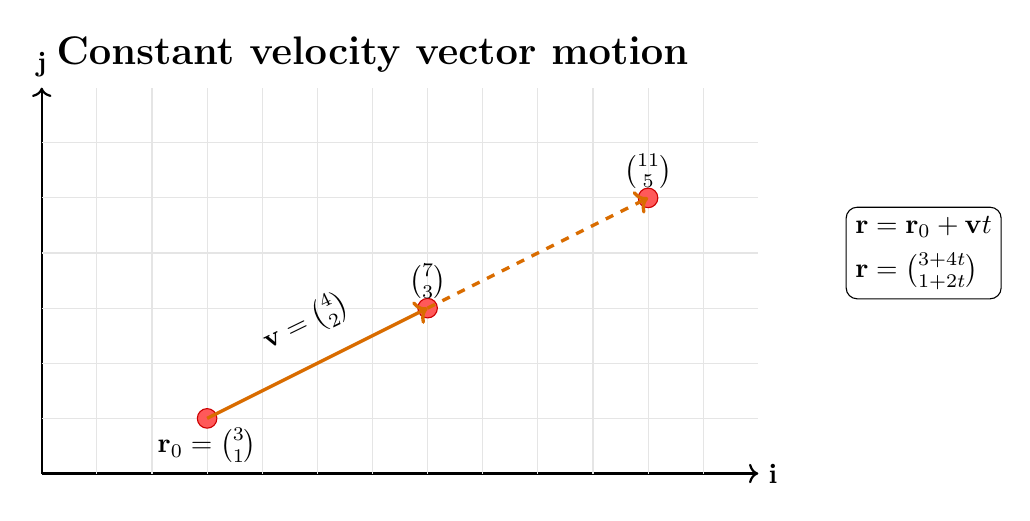
\begin{tikzpicture}[scale=0.7, axis/.style={->, thick}, motion/.style={->, very thick, orange!85!black}, point/.style={circle, fill=red!65, draw=red!80!black, inner sep=2.5pt}]
\node[font=\bfseries\Large] at (6,7.6) {Constant velocity vector motion};
\draw[axis] (0,0)--(13,0) node[right] {$\mathbf i$};
\draw[axis] (0,0)--(0,7) node[above] {$\mathbf j$};
\foreach \x in {1,...,12} \draw[gray!20] (\x,0)--(\x,7);
\foreach \y in {1,...,6} \draw[gray!20] (0,\y)--(13,\y);
\coordinate (R0) at (3,1); \coordinate (R1) at (7,3); \coordinate (R2) at (11,5);
\node[point] at (R0) {}; \node[point] at (R1) {}; \node[point] at (R2) {};
\draw[motion] (R0)--(R1); \draw[motion,dashed] (R1)--(R2);
\node[below] at (R0) {$\mathbf r_0=\binom{3}{1}$};
\node[above] at (R1) {$\binom{7}{3}$}; \node[above] at (R2) {$\binom{11}{5}$};
\node[rotate=26, above] at (5,2.3) {$\mathbf v=\binom{4}{2}$};
\node[draw, rounded corners, fill=white, align=left] at (16,4) {$\mathbf r=\mathbf r_0+\mathbf vt$\\[4pt]$\mathbf r=\binom{3+4t}{1+2t}$};
\end{tikzpicture}
\end{document}
